\section{Logistická regrese}\label{sec:logisticka}

Logistická regrese je přes svůj název \emph{klasifikační} model: lineární funkci vstupu protáhne \emph{logistickou (sigmoidní)} funkcí a~výstup čte jako \emph{pravděpodobnost} třídy. Je to jedna z~nejpoužívanějších klasifikačních technik a~zároveň nejjednodušší \emph{pravděpodobnostní} klasifikátor trénovaný \emph{maximum likelihood estimation} (MLE, maximální věrohodnost; sekce~\ref{sec:evaluace}). V~této sekci ji zavedeme pro binární klasifikaci, odvodíme její ztrátovou funkci i~gradient a~zobecníme ji softmaxem na více tříd.

\begin{poznamka}[Vztah k~S1]
Okruh S1 (sekce \emph{Strojové učení}) zmiňuje logistickou regresi přehledově jako „změkčený tvrdý práh`` s~pravděpodobnostním výstupem. Zde to \textbf{nezdvojujeme} -- jdeme do hloubky, kterou S1 přenechává S3: parametrizace přes sigmoid, ztráta jako negativní log-věrohodnost, odvození gradientu a~SGD, multiclass softmax.
\end{poznamka}

\subsection{Binární logistická regrese}

\subsubsection*{Od tvrdého prahu k~sigmoidě}

Lineární klasifikátor počítá skóre $\bar y(\mathbf{x};\mathbf{w})=\mathbf{w}^{\!\top}\mathbf{x}+b$ a~třídu přiřadí podle znaménka (prahu). \emph{Perceptron} (historicky nejstarší algoritmus, Rosenblatt 1958) používá \emph{tvrdý} práh $\sign(\bar y)$: vrací jen třídu $\{-1,+1\}$, na lineárně neseparabilních datech nekonverguje a~nedává pravděpodobnosti. Logistická regrese tvrdý práh \emph{změkčí} -- skóre $\bar y$ protáhne \textbf{sigmoidou} a~výstup interpretuje jako $P(C_1\mid\mathbf{x})$.

\begin{definice}[Sigmoidní (logistická) funkce]
\emph{Sigmoida} je funkce
\[ \sigma(z)=\frac{1}{1+e^{-z}}. \]
Má hodnoty v~otevřeném intervalu $(0,1)$, je rostoucí, $\sigma(0)=\tfrac12$, $\sigma(-z)=1-\sigma(z)$ (středová symetrie kolem bodu $(0,\tfrac12)$) a~asymptoticky $\sigma(z)\to 1$ pro $z\to+\infty$, $\sigma(z)\to 0$ pro $z\to-\infty$. Její derivace je
\[ \sigma'(z)=\sigma(z)\big(1-\sigma(z)\big),\qquad \sigma'(0)=\tfrac14. \]
\end{definice}

\begin{center}
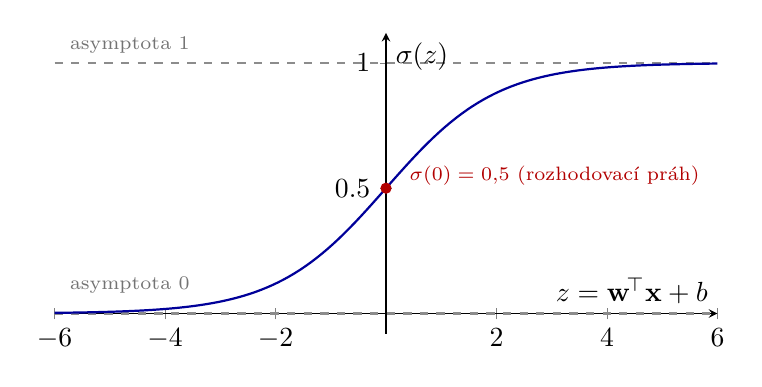
\begin{tikzpicture}
\begin{axis}[width=10cm,height=5.4cm,
  xlabel={$z=\mathbf{w}^{\!\top}\mathbf{x}+b$},ylabel={$\sigma(z)$},
  xmin=-6,xmax=6,ymin=-0.08,ymax=1.12,
  xtick={-6,-4,-2,0,2,4,6},ytick={0,0.5,1},
  axis lines=middle,every axis plot/.append style={thick},clip=false,
  enlargelimits=false]
  % asymptoty
  \addplot[black!45,dashed,domain=-6:6,samples=2]{1};
  \addplot[black!45,dashed,domain=-6:6,samples=2]{0};
  \node[font=\scriptsize,black!55,anchor=south west] at (axis cs:-5.9,1) {asymptota $1$};
  \node[font=\scriptsize,black!55,anchor=south west] at (axis cs:-5.9,0.04) {asymptota $0$};
  % sigmoida
  \addplot[blue!60!black,domain=-6:6,samples=120]{1/(1+exp(-x))};
  % bod 0.5
  \addplot[only marks,mark=*,mark size=1.6pt,red!70!black] coordinates {(0,0.5)};
  \node[font=\scriptsize,red!70!black,anchor=west] at (axis cs:0.25,0.55) {$\sigma(0)=0{,}5$ (rozhodovací práh)};
\end{axis}
\end{tikzpicture}
\obrpopis{Sigmoida $\sigma(z)=1/(1+e^{-z})$. Hladce přechází z~$0$ do~$1$, hodnotu $0{,}5$ nabývá v~$z=0$ (rozhodovací práh) a~k~asymptotám $0$ a~$1$ se blíží pro velká záporná, resp.\ kladná $z$. Záporné $z$ tedy znamená pravděpodobnost třídy $C_1$ pod $50\,\%$, kladné nad $50\,\%$.}
\end{center}

\begin{definice}[Model binární logistické regrese]
Pro binární klasifikaci ($t\in\{0,1\}$) logistická regrese modeluje podmíněnou pravděpodobnost pozitivní třídy $C_1$ pomocí lineární funkce protažené sigmoidou. Označíme \emph{lineární část} $\bar y(\mathbf{x};\mathbf{w})=\mathbf{w}^{\!\top}\mathbf{x}$ a~celkový výstup
\[ y(\mathbf{x};\mathbf{w})=\sigma\big(\mathbf{w}^{\!\top}\mathbf{x}\big),\qquad
   P(C_1\mid\mathbf{x})=y(\mathbf{x};\mathbf{w}),\qquad
   P(C_0\mid\mathbf{x})=1-y(\mathbf{x};\mathbf{w}). \]
\textbf{Predikce.} Vstup zařadíme do třídy $C_1$, je-li $y(\mathbf{x};\mathbf{w})\ge 0{,}5$ (\emph{rozhodovací práh} $0{,}5$), jinak do $C_0$. Protože $\sigma(z)\ge\tfrac12 \iff z\ge 0$, je rozhodnutí ekvivalentní podmínce $\mathbf{w}^{\!\top}\mathbf{x}\ge 0$.
\end{definice}

\begin{intuice}[Bias jako práh; lineární rozhodovací hranice]
\emph{Bias} $b$ (absorbovaný do $\mathbf{w}$ přidáním stálého příznaku $x_0=1$, jak děláme dál) hraje roli trénovatelného prahu, proto stačí porovnávat skóre s~nulou. \textbf{Rozhodovací hranice} je množina bodů s~$y=0{,}5$, tj.\ $\mathbf{w}^{\!\top}\mathbf{x}=0$ -- to je \emph{nadrovina} (přímka v~2D), takže logistická regrese je \emph{lineární} klasifikátor. Sigmoida mění jen \emph{tvar} přechodu mezi třídami (jak rychle pravděpodobnost roste přes hranici), ne jeho \emph{polohu}.
\end{intuice}

\begin{poznamka}[Logit jako log-šance]
Inverze sigmoidy dává pro $p=P(C_1\mid\mathbf{x})$ lineární část jako \emph{logit}:
\[ \bar y(\mathbf{x};\mathbf{w})=\log\frac{p}{1-p}=\log\frac{P(C_1\mid\mathbf{x})}{P(C_0\mid\mathbf{x})}. \]
Lineární skóre tak má význam \emph{logaritmu šance} (log-odds) mezi oběma třídami: $\bar y>0$ znamená šanci ve prospěch $C_1$, $\bar y<0$ ve prospěch $C_0$.
\end{poznamka}

\subsection{Ztrátová funkce, gradient a~SGD}

\subsubsection*{Ztráta = negativní log-věrohodnost (křížová entropie)}

Logistická regrese se trénuje \emph{maximum likelihood estimation} (MLE) (sekce~\ref{sec:evaluace}). Výstup $y(\mathbf{x};\mathbf{w})$ je přímo pravděpodobnost třídy $C_1$, takže cíl $t$ pochází z~\emph{Bernoulliho} rozdělení s~parametrem $\varphi=y$: $p(t\mid\mathbf{x};\mathbf{w})=y^{\,t}(1-y)^{1-t}$. Minimalizujeme \emph{negativní logaritmickou věrohodnost} (NLL); pro minibatch $N$ příkladů je ztráta
\[ E(\mathbf{w})=\frac1N\sum_{i=1}^N -\log p\big(C_{t_i}\mid\mathbf{x}_i;\mathbf{w}\big)
   =\frac1N\sum_{i=1}^N \Big(-t_i\log y(\mathbf{x}_i;\mathbf{w})-(1-t_i)\log\big(1-y(\mathbf{x}_i;\mathbf{w})\big)\Big). \]

\begin{definice}[Binární křížová entropie]
Pro jeden příklad s~výstupem $y=\sigma(\mathbf{w}^{\!\top}\mathbf{x})$ a~cílem $t\in\{0,1\}$ je ztráta (binární křížová entropie, $=$ NLL Bernoulliho modelu)
\[ E = -t\log y-(1-t)\log(1-y). \]
\end{definice}

\begin{intuice}
Pro $t=1$ se z~ní stane $-\log y$ (chceme $y\to 1$), pro $t=0$ je to $-\log(1-y)$ (chceme $y\to 0$). Jistá \emph{a~správná} predikce dá ztrátu $0$; jistá \emph{a~chybná} predikce ($y\to 0$ při $t=1$) ztrátu $+\infty$ -- model je za sebevědomý omyl tvrdě penalizován. Název „křížová entropie`` plyne z~obecného rámce MLE: NLL $=$ křížová entropie mezi empirickým rozdělením cílů a~modelem (sekce~\ref{sec:evaluace}). Pozn.: kvadratická (MSE) ztráta se zde \emph{nepoužívá} -- vede k~nekonvexnímu problému a~mizejícím gradientům v~saturaci sigmoidy.
\end{intuice}

\subsubsection*{Odvození gradientu}

Toto odvození žádá otázka SZZ jaro 2025 (č.~29, část~2). Provedeme derivaci krok po kroku pro \emph{jeden} příklad; značme $z=\mathbf{w}^{\!\top}\mathbf{x}$, takže $y=\sigma(z)$ a~$E=-t\log\sigma(z)-(1-t)\log\big(1-\sigma(z)\big)$. Cílem je $\nabla_{\mathbf{w}}E$.

\begin{veta}[Gradient ztráty logistické regrese]
Pro jeden příklad $(\mathbf{x},t)$ a~ztrátu $E=-t\log\sigma(\mathbf{w}^{\!\top}\mathbf{x})-(1-t)\log\big(1-\sigma(\mathbf{w}^{\!\top}\mathbf{x})\big)$ platí
\[ \frac{\partial E}{\partial z}=\sigma(z)-t,\qquad\text{a~tedy}\qquad
   \boxed{\ \nabla_{\mathbf{w}}E=\big(\sigma(\mathbf{w}^{\!\top}\mathbf{x})-t\big)\,\mathbf{x}\ }. \]
\end{veta}

\begin{proof}[Odvození \textnormal{(krok po kroku)}]
\hfill\par
\begin{enumerate}[label=(\arabic*)]
  \item \textbf{Derivace sigmoidy.} Z~$\sigma(z)=\big(1+e^{-z}\big)^{-1}$ řetízkovým pravidlem
    \[ \sigma'(z)=-\big(1+e^{-z}\big)^{-2}\cdot(-e^{-z})=\frac{e^{-z}}{(1+e^{-z})^2}
       =\frac{1}{1+e^{-z}}\cdot\frac{e^{-z}}{1+e^{-z}}=\sigma(z)\big(1-\sigma(z)\big), \]
    kde poslední rovnost využívá $\dfrac{e^{-z}}{1+e^{-z}}=\dfrac{(1+e^{-z})-1}{1+e^{-z}}=1-\sigma(z)$.
  \item \textbf{Derivace ztráty podle $z$.} Použijeme $\dfrac{\partial}{\partial z}\log\sigma=\dfrac{\sigma'}{\sigma}$ a~$\dfrac{\partial}{\partial z}\log(1-\sigma)=\dfrac{-\sigma'}{1-\sigma}$:
    \[ \frac{\partial E}{\partial z}
       = -t\cdot\frac{\sigma'(z)}{\sigma(z)}-(1-t)\cdot\frac{-\sigma'(z)}{1-\sigma(z)}
       = -t\,\frac{\sigma'(z)}{\sigma(z)}+(1-t)\,\frac{\sigma'(z)}{1-\sigma(z)}. \]
  \item \textbf{Dosazení $\sigma'=\sigma(1-\sigma)$.} V~prvním zlomku se zkrátí $\sigma$, ve druhém $(1-\sigma)$:
    \[ \frac{\partial E}{\partial z}
       = -t\,\big(1-\sigma(z)\big)+(1-t)\,\sigma(z). \]
  \item \textbf{Roznásobení a~zjednodušení.}
    \[ \frac{\partial E}{\partial z}
       = -t+t\,\sigma(z)+\sigma(z)-t\,\sigma(z)
       = \sigma(z)-t. \]
    Členy $\pm t\,\sigma(z)$ se vyruší; zbývá rozdíl predikce a~cíle.
  \item \textbf{Přechod ke gradientu podle $\mathbf{w}$.} Protože $z=\mathbf{w}^{\!\top}\mathbf{x}$, je $\nabla_{\mathbf{w}}z=\mathbf{x}$. Řetízkovým pravidlem
    \[ \nabla_{\mathbf{w}}E=\frac{\partial E}{\partial z}\,\nabla_{\mathbf{w}}z=\big(\sigma(z)-t\big)\,\mathbf{x}=\big(y(\mathbf{x};\mathbf{w})-t\big)\,\mathbf{x}. \qedhere \]
\end{enumerate}
\end{proof}

\begin{intuice}[Elegantní tvar a~jednotnost s~lineární regresí]
Gradient má pozoruhodně jednoduchý tvar \emph{(chyba predikce)} $\times$ \emph{(vstup)}: $\big(y-t\big)\mathbf{x}$. Je-li predikce přesná ($y=t$), gradient je nulový a~váhy se nemění; čím větší chyba, tím větší krok, a~to ve směru příznaků $\mathbf{x}$. \emph{Stejný} tvar $\big(y-t\big)\mathbf{x}$ má gradient \emph{lineární} regrese s~MSE ztrátou (sekce~\ref{sec:linreg}) i~\emph{softmaxové} regrese (níže) -- to není náhoda, ale důsledek \emph{zobecněných lineárních modelů}: vhodná aktivace (identita / sigmoida / softmax) s~odpovídajícím rozdělením (normální / Bernoulli / kategorické) a~NLL ztrátou vždy vede k~témuž tvaru gradientu.
\end{intuice}

\subsubsection*{Stochastický gradientní sestup}

Minimum ztráty nemá logistická regrese (na rozdíl od lineární) v~uzavřeném tvaru, hledáme ho proto \emph{gradientním sestupem}. V~praxi \emph{stochastickým} (SGD): místo plného gradientu přes všechna data použijeme odhad z~jednoho příkladu nebo malé dávky (minibatch).

\begin{algo}[Trénování logistické regrese (minibatch SGD)]
\textbf{Vstup:} data $(\mathbf{X}\in\mathbb{R}^{N\times D},\ \mathbf{t}\in\{0,1\}^N)$, rychlost učení $\alpha>0$.\par
\textbf{Výstup:} váhy $\mathbf{w}$.
\begin{enumerate}[label=\arabic*.,leftmargin=2.2em]
  \item $\mathbf{w}\leftarrow\mathbf{0}$ (nebo malé náhodné hodnoty) \cmt{inicializace}
  \item \textbf{opakuj} do konvergence (nebo vyčerpání trpělivosti) pro minibatch $\mathbb{B}$:
  \begin{enumerate}[label=\alph*),leftmargin=2.2em]
    \item $\displaystyle \mathbf{g}\leftarrow\frac{1}{|\mathbb{B}|}\sum_{i\in\mathbb{B}}\big(\sigma(\mathbf{w}^{\!\top}\mathbf{x}_i)-t_i\big)\,\mathbf{x}_i$ \cmt{průměrný gradient na dávce}
    \item $\mathbf{w}\leftarrow\mathbf{w}-\alpha\,\mathbf{g}$ \cmt{krok proti gradientu}
  \end{enumerate}
\end{enumerate}
\end{algo}

\noindent Pro jeden příklad (čistý SGD, $|\mathbb{B}|=1$) je krok přímo
\[ \mathbf{w}\leftarrow\mathbf{w}-\alpha\big(\sigma(\mathbf{w}^{\!\top}\mathbf{x})-t\big)\,\mathbf{x}. \]

\begin{poznamka}[Prevence overfittingu]
Vše, co platí o~\emph{příznacích} a~$L^2$ \emph{regularizaci} obecně, platí i~zde (sekce~\ref{sec:preuceni}). Overfittingu (přeučení) při SGD bráníme zejména:
\begin{itemize}
  \item \textbf{$L^2$ regularizací} -- ke ztrátě přidáme $\tfrac{\lambda}{2}\|\mathbf{w}\|^2$, čímž do kroku přibude člen $-\alpha\lambda\mathbf{w}$ (váhy se v~každém kroku mírně „smršťují`` k~nule);
  \item \textbf{early stopping} (včasné zastavení) -- sledujeme \emph{validační} chybu a~trénování ukončíme, jakmile začne růst (model se přestává učit signál a~začíná se učit šum).
\end{itemize}
Pomáhá i~rozumný \emph{learning-rate schedule} (postupné snižování $\alpha$). Podrobnosti a~obrázek validační vs.\ trénovací chyby viz sekce~\ref{sec:preuceni}.
\end{poznamka}

\subsection{Klasifikace do více tříd: softmax}

Pro $K>2$ tříd zobecníme model dvěma kroky: vygenerujeme $K$ lineárních výstupů (každý se svými vahami) a~sigmoidu nahradíme \textbf{softmaxem}, který $K$ čísel převede na rozdělení pravděpodobností přes třídy.

\begin{definice}[Multinomiální logistická regrese (softmax)]
Pro $K$ tříd máme matici vah $\mathbf{W}\in\mathbb{R}^{D\times K}$ (sloupec na třídu). Lineární část je vektor $\bar{\mathbf{y}}(\mathbf{x};\mathbf{W})=\mathbf{x}^{\!\top}\mathbf{W}\in\mathbb{R}^K$ (jeho $i$-tá složka je skóre třídy $C_i$). \emph{Softmax} z~něj dělá pravděpodobnosti:
\[ P(C_i\mid\mathbf{x};\mathbf{W})=\operatorname{softmax}\big(\bar{\mathbf{y}}\big)_i=\frac{e^{\bar y_i}}{\sum_{j=0}^{K-1} e^{\bar y_j}}. \]
Výsledné hodnoty jsou v~$(0,1)$ a~sčítají se na~$1$. Klasifikujeme do třídy s~\emph{nejvyšší} pravděpodobností, $\hat c=\argmax_i P(C_i\mid\mathbf{x};\mathbf{W})$. Model se též nazývá \emph{softmax regrese} nebo \emph{maximum entropy} klasifikátor.
\end{definice}

\begin{intuice}[Softmax zobecňuje sigmoidu]
Softmax je „měkký argmax``: zvýrazní největší skóre, ale zachová pravděpodobnostní rozdělení (nejen tvrdé vítězství). Pro $K=2$ se redukuje na sigmoidu, $\sigma(z)=\operatorname{softmax}\big([z,0]\big)_0=\dfrac{e^{z}}{e^{z}+e^{0}}=\dfrac{1}{1+e^{-z}}$. Exponenciála je vždy kladná, dělení normalizuje na součet~$1$. Softmax je invariantní vůči přičtení konstanty ke všem skóre ($\operatorname{softmax}(\bar{\mathbf{y}}+c)=\operatorname{softmax}(\bar{\mathbf{y}})$), takže model je mírně \emph{přeurčený} -- pro $K$ tříd by stačilo $K-1$ sad vah.
\end{intuice}

\begin{poznamka}[Ztráta a~trénování -- analogicky binárnímu případu]
Cíl $t\in\{0,1,\dots,K-1\}$ reprezentujeme \emph{one-hot} vektorem $\mathbf{1}_t$ ($1$ na pozici správné třídy, jinak $0$). Cíl pochází z~\emph{kategorického} rozdělení, ztráta je opět NLL $=$ (kategorická) křížová entropie:
\[ E(\mathbf{W})=\frac1N\sum_{i=1}^N -\log P\big(C_{t_i}\mid\mathbf{x}_i;\mathbf{W}\big). \]
Trénuje se stejným minibatch SGD jako binární případ. Gradient ztráty podle vah třídy má opět tvar \emph{(chyba) $\times$ (vstup)},
\[ \nabla_{\mathbf{W}}E=\mathbf{x}\,\big(\mathbf{y}(\mathbf{x})-\mathbf{1}_t\big)^{\!\top}\in\mathbb{R}^{D\times K}\quad\text{(pro jeden příklad; sloupec třídy $i$ je $(y_i-[t{=}i])\,\mathbf{x}$)}, \]
kde $\mathbf{y}(\mathbf{x})=\operatorname{softmax}(\mathbf{x}^{\!\top}\mathbf{W})$ je vektor predikovaných pravděpodobností. Odvození je analogické binárnímu případu: derivace křížové entropie podle skóre softmaxu vyjde $\partial E/\partial\bar{\mathbf{y}}=\mathbf{y}(\mathbf{x})-\mathbf{1}_t$. Rozhodovací oblasti softmaxu jsou \emph{konvexní} (a~tedy souvislé): hranice mezi dvojicemi tříd jsou lineární.
\end{poznamka}

\subsection{Řešené příklady}

\begin{priklad}[SZZ léto 2022 č.~10: Predikční funkce logistické regrese]
\szzotazka{léto 2022}{10}{Logistická regrese}\par
\textbf{Zadání.} \textbf{(1)}~Napište funkci, kterou predikuje model logistické regrese. \textbf{(2)}~Jakých hodnot tato funkce nabývá a~jaká je jejich interpretace?

\smallskip
\textbf{Řešení.} \textbf{(1)}~Model spočítá lineární kombinaci příznaků $z=\mathbf{w}^{\!\top}\mathbf{x}+b$ a~aplikuje na ni logistickou (sigmoidní) funkci $\sigma(z)=\tfrac{1}{1+e^{-z}}$, takže predikuje
\[ \hat y=\sigma\!\big(\mathbf{w}^{\!\top}\mathbf{x}+b\big)=\frac{1}{1+e^{-(\mathbf{w}^{\!\top}\mathbf{x}+b)}}. \]
\textbf{(2)}~Hodnoty leží v~intervalu $(0,1)$ a~interpretují se jako pravděpodobnost příslušnosti k~pozitivní třídě, $P(y{=}1\mid\mathbf{x})$. Vlastní klasifikaci dostaneme prahováním (typicky práh $0{,}5$: třída $1$ pro $\hat y\ge 0{,}5$, jinak třída $0$).
\end{priklad}

\begin{priklad}[SZZ jaro 2025 č.~29: Logistická regrese pro binární klasifikaci]
\szzotazka{jaro 2025}{29}{Logistická regrese pro binární klasifikaci}\par
\textbf{Zadání.} Dataset $\mathbf{X}=(\mathbf{x}_1,\dots,\mathbf{x}_N)$ s~cíli $\mathbf{t}=(t_1,\dots,t_N)$. \textbf{(1)}~Jak použít logistickou regresi pro binární klasifikaci? Jak vypadá predikce? Jak nezávisle odhadnout chybu na neviděných datech? \textbf{(2)}~Jak je definována ztrátová funkce? \emph{Odvoďte} její derivaci a~ukažte SGD. \textbf{(3)}~Jak při SGD zabráníte overfittingu?

\smallskip
\textbf{Řešení.}

\textbf{(1)~Model a~predikce.} Logistická regrese modeluje $P(C_1\mid\mathbf{x})=y(\mathbf{x};\mathbf{w})=\sigma(\mathbf{w}^{\!\top}\mathbf{x})$ s~$\sigma(z)=1/(1+e^{-z})$ a~$P(C_0\mid\mathbf{x})=1-y$. \emph{Predikce:} třída $1$, je-li $y\ge 0{,}5$ (ekvivalentně $\mathbf{w}^{\!\top}\mathbf{x}\ge 0$), jinak třída $0$. \emph{Odhad chyby na neviděných datech:} data rozdělíme na \emph{trénovací} (učení vah), \emph{validační} (ladění hyperparametrů, např.\ $\lambda$, rozhodnutí o~early stopping) a~\emph{testovací} (jediné finální měření). Při málu dat použijeme $k$-násobnou křížovou validaci (sekce~\ref{sec:evaluace}).

\textbf{(2)~Ztráta, derivace, SGD.} Ztráta je negativní log-věrohodnost (Bernoulli), pro minibatch
\[ E(\mathbf{w})=\frac1N\sum_i -\log p\big(C_{t_i}\mid\mathbf{x}_i;\mathbf{w}\big),\qquad
   \text{pro 1 vzor}\ E=-t\log\sigma(z)-(1-t)\log\big(1-\sigma(z)\big),\ z=\mathbf{w}^{\!\top}\mathbf{x}. \]
Derivaci provedeme přes $\sigma'(z)=\sigma(z)\big(1-\sigma(z)\big)$:
\[
\frac{\partial E}{\partial z}
= -t\frac{\sigma'}{\sigma}+(1-t)\frac{\sigma'}{1-\sigma}
= -t(1-\sigma)+(1-t)\sigma
= -t+t\sigma+\sigma-t\sigma
= \sigma(z)-t,
\]
a~protože $\nabla_{\mathbf{w}}z=\mathbf{x}$, je $\nabla_{\mathbf{w}}E=\big(\sigma(\mathbf{w}^{\!\top}\mathbf{x})-t\big)\mathbf{x}$ (plné odvození viz věta výše). \emph{SGD:} inicializuj $\mathbf{w}$, opakuj $\mathbf{w}\leftarrow\mathbf{w}-\alpha\big(\sigma(\mathbf{w}^{\!\top}\mathbf{x}_i)-t_i\big)\mathbf{x}_i$ (resp.\ průměr přes minibatch).

\textbf{(3)~Prevence overfittingu.} $L^2$ regularizace (člen $\tfrac{\lambda}{2}\|\mathbf{w}\|^2$ ke ztrátě, ve kroku $-\alpha\lambda\mathbf{w}$), \emph{early stopping} (zastavit, když roste validační chyba) a~rozumný learning-rate schedule (sekce~\ref{sec:preuceni}).
\end{priklad}

\begin{priklad}[SZZ podzim 2024 č.~29: Logistická regrese (model, výstup, multiclass)]
\szzotazka{podzim 2024}{29}{Logistická regrese}\par
\textbf{Zadání.} Model má předpovídat pravděpodobnost úspěchu u~zkoušky podle doby učení; data (úspěch $1$ / neúspěch $0$ vs.\ doba učení) jsou na obrázku. \textbf{(1)}~Popište model logistické regrese: jak se spočítá výstup, jak se trénují parametry, jaká je ztrátová funkce? \textbf{(2)}~Zakreslete přibližně výstup natrénovaného modelu (nepočítejte). \textbf{(3)}~Jak by se model lišil při klasifikaci do více než dvou tříd (např.\ predikce známky)?

\smallskip
\textbf{Řešení.}

\textbf{(1)~Model.} Jeden příznak $x=$ doba učení (plus bias). Výstup $y(x;\mathbf{w})=\sigma(w_1 x+w_0)$, čtený jako $P(\text{úspěch}\mid x)$; klasifikace prahem $0{,}5$. \emph{Trénink:} maximum likelihood estimation (MLE) přes SGD, minimalizujeme \emph{negativní log-věrohodnost} (NLL, binární křížovou entropii) $E=-t\log y-(1-t)\log(1-y)$ s~gradientem $\big(y-t\big)\,\mathbf{x}$; krok $\mathbf{w}\leftarrow\mathbf{w}-\alpha\,\mathbf{g}$.

\textbf{(2)~Výstup modelu.} Sigmoidní křivka rostoucí s~dobou učení: u~krátké doby blízko~$0$, u~dlouhé blízko~$1$, hodnotu $0{,}5$ (rozhodovací práh) protíná zhruba tam, kde se v~datech mísí neúspěchy a~úspěchy.

\begin{center}
\begin{tikzpicture}
\begin{axis}[width=10cm,height=5.2cm,
  xlabel={doba učení [h]},ylabel={$P(\text{úspěch})$},
  xmin=0,xmax=10,ymin=-0.12,ymax=1.15,
  xtick={0,2,4,6,8,10},ytick={0,0.5,1},
  axis lines=left,every axis plot/.append style={thick},clip=false,
  enlargelimits=false]
  % prahova cara 0.5
  \addplot[black!40,dashed,domain=0:10,samples=2]{0.5};
  \node[font=\scriptsize,black!55,anchor=south east] at (axis cs:10,0.5) {práh $0{,}5$};
  % sigmoidni vystup: stred okolo x=5, sklon 1.1
  \addplot[blue!60!black,domain=0:10,samples=120]{1/(1+exp(-1.1*(x-5)))};
  \node[font=\scriptsize,blue!60!black,anchor=west] at (axis cs:6.2,0.78) {výstup modelu};
  % data: neuspechy (t=0) pri kratke dobe, uspechy (t=1) pri dlouhe
  \addplot[only marks,mark=*,mark size=2pt,red!70!black] coordinates {(1,0)(1.8,0)(2.4,0)(3,0)(3.6,0)(4.4,0)(5.2,0)};
  \addplot[only marks,mark=*,mark size=2pt,green!45!black] coordinates {(4.8,1)(5.6,1)(6.2,1)(7,1)(7.6,1)(8.4,1)(9.2,1)};
  \node[font=\scriptsize,red!70!black,anchor=south west] at (axis cs:0.2,0.07) {neúspěch ($t=0$)};
  \node[font=\scriptsize,green!45!black,anchor=south west] at (axis cs:0.2,1.04) {úspěch ($t=1$)};
\end{axis}
\end{tikzpicture}
\obrpopis{Logistická regrese na 1D datech (doba učení $\to$ úspěch). Body leží na $y=0$ (neúspěchy, krátká doba) a~$y=1$ (úspěchy, dlouhá doba); modrá sigmoida je výstup modelu $P(\text{úspěch}\mid x)$. Práh $0{,}5$ protíná v~pásmu, kde se obě třídy překrývají -- to je rozhodovací hranice. Data jsou schematická.}
\end{center}

\textbf{(3)~Více tříd.} Místo jednoho výstupu se sigmoidou bychom měli $K$ výstupů (sada vah na třídu) a~sigmoidu nahradili \emph{softmaxem} $P(C_i\mid\mathbf{x})=e^{\bar y_i}/\sum_j e^{\bar y_j}$, který dá rozdělení pravděpodobností přes $K$ tříd (sčítá se na~$1$). Predikce $=\argmax_i P(C_i\mid\mathbf{x})$, ztráta $=$ kategorická křížová entropie, trénink opět SGD. (Pro predikci \emph{známky} by navíc dávalo smysl využít její \emph{uspořádanost} -- ordinální regrese -- ale to už je nad rámec.)
\end{priklad}
